% ============================================================
%  DISCOVERY CURRICULUM — Journey 2, Module 6
%  "Multivariable Calculus"
%  Compile with: pdflatex J2_M6.tex  (run twice for references)
% ============================================================

\documentclass[12pt, a4paper]{article}

\usepackage[a4paper, top=2.5cm, bottom=2.5cm, left=2.8cm, right=2.8cm, headheight=15pt]{geometry}
\usepackage{amsmath, amssymb, amsthm}
\usepackage{xcolor}
\usepackage{mdframed}
\usepackage{enumitem}
\usepackage{tikz}
\usetikzlibrary{arrows.meta, positioning, calc}
\usepackage{pgfplots}
\pgfplotsset{compat=1.18}
\usepackage{booktabs}
\usepackage{fancyhdr}
\usepackage{titlesec}
\usepackage{parskip}
\usepackage{hyperref}
\hypersetup{colorlinks=true, linkcolor=NavyBlue, urlcolor=NavyBlue}

% ── Colours ─────────────────────────────────────────────────
\definecolor{NavyBlue}{HTML}{1A3A5C}
\definecolor{MidBlue}{HTML}{2E6DA4}
\definecolor{Gold}{HTML}{C8922A}
\definecolor{LightBlue}{HTML}{EBF2FA}
\definecolor{LightGold}{HTML}{FDF4E3}
\definecolor{DarkGrey}{HTML}{3A3A3A}
\definecolor{BoxGreen}{HTML}{E8F5E9}
\definecolor{SidebarGrey}{HTML}{F5F5F5}

% ── Section formatting ───────────────────────────────────────
\titleformat{\section}{\Large\bfseries\color{NavyBlue}}{}{0em}{}[{\color{MidBlue}\vspace{2pt}\rule{\linewidth}{1.5pt}}]
\titleformat{\subsection}{\large\bfseries\color{MidBlue}}{}{0em}{}

% ── Header / Footer ─────────────────────────────────────────
\pagestyle{fancy}
\fancyhf{}
\fancyhead[L]{\small\color{DarkGrey}\textit{Discovery Curriculum}}
\fancyhead[R]{\small\color{DarkGrey}\textit{Journey 2 $\cdot$ Module 6}}
\fancyfoot[C]{\small\color{MidBlue}\thepage}
\renewcommand{\headrulewidth}{0.4pt}

% ── Environments ─────────────────────────────────────────────
\newmdenv[
  backgroundcolor=NavyBlue!7,
  linecolor=NavyBlue, linewidth=2pt,
  leftline=true, rightline=false, topline=false, bottomline=false,
  innerleftmargin=14pt, innerrightmargin=10pt,
  innertopmargin=10pt, innerbottommargin=10pt,
  skipabove=14pt, skipbelow=10pt
]{puzzlebox}

\newmdenv[
  backgroundcolor=LightGold,
  linecolor=Gold, linewidth=2pt,
  leftline=true, rightline=false, topline=false, bottomline=false,
  innerleftmargin=14pt, innerrightmargin=10pt,
  innertopmargin=10pt, innerbottommargin=10pt,
  skipabove=14pt, skipbelow=10pt
]{discoverybox}

\newmdenv[
  backgroundcolor=LightBlue,
  linecolor=MidBlue, linewidth=1.5pt,
  roundcorner=4pt,
  innerleftmargin=14pt, innerrightmargin=10pt,
  innertopmargin=10pt, innerbottommargin=10pt,
  skipabove=14pt, skipbelow=10pt
]{namebox}

\newmdenv[
  backgroundcolor=BoxGreen,
  linecolor=DarkGrey!35, linewidth=1pt,
  roundcorner=4pt,
  innerleftmargin=14pt, innerrightmargin=10pt,
  innertopmargin=10pt, innerbottommargin=10pt,
  skipabove=14pt, skipbelow=10pt
]{reflectionbox}

\newmdenv[
  backgroundcolor=SidebarGrey,
  linecolor=Gold, linewidth=1.2pt,
  leftline=true, rightline=false, topline=false, bottomline=false,
  innerleftmargin=12pt, innerrightmargin=10pt,
  innertopmargin=7pt, innerbottommargin=7pt,
  skipabove=10pt, skipbelow=10pt
]{thought}

\newcounter{problem}
\newenvironment{problem}[1][]{%
  \refstepcounter{problem}%
  \par\vspace{6pt}%
  \noindent\textbf{\color{MidBlue}Problem \theproblem}%
  \ifx&#1&\else\ \textit{(#1)}\fi\textbf{.}\enskip
}{\par\vspace{4pt}}

\newcounter{deepproblem}
\newenvironment{deepproblem}[1][]{%
  \refstepcounter{deepproblem}%
  \par\vspace{6pt}%
  \noindent\textbf{\color{NavyBlue}$\bigstar$\ Deep Problem \thedeepproblem}%
  \ifx&#1&\else\ \textit{(#1)}\fi\textbf{.}\enskip
}{\par\vspace{4pt}}

% ============================================================
\begin{document}
no% ============================================================

\thispagestyle{empty}
\begin{center}
{\small\color{MidBlue}\textbf{DISCOVERY CURRICULUM}\quad$\cdot$\quad\textbf{JOURNEY 2: CHANGE}}

\vspace{0.6cm}
{\color{NavyBlue}\rule{\linewidth}{2pt}}
\vspace{0.5cm}

{\Huge\bfseries\color{NavyBlue}Module 6}\\[0.3cm]
{\LARGE\bfseries\color{MidBlue}Multivariable Calculus}\\[0.4cm]
{\color{Gold}\rule{0.4\linewidth}{1.2pt}}\\[0.4cm]
{\large\itshape\color{DarkGrey}
In one dimension, a derivative is a number.\\[0.15cm]
In higher dimensions, it becomes a direction.}

\vspace{1cm}
\begin{tabular}{rl}
\color{DarkGrey}\textbf{Journey}           & Journey 2 --- Change \\[4pt]
\color{DarkGrey}\textbf{Module}            & 6 of 6 \textit{(final module of Journey 2)} \\[4pt]
\color{DarkGrey}\textbf{Prerequisites}     & J2 Modules 1--5; J1 Modules 1--3 (functions, vectors) \\[4pt]
\color{DarkGrey}\textbf{You will discover} & Partial derivatives, gradient, chain rule in higher dimensions, double integrals \\[4pt]
\color{DarkGrey}\textbf{Format}            & 8 problems $+$ 3 deep problems $\approx$ 14 pages \\
\end{tabular}

\vspace{1cm}
{\color{NavyBlue}\rule{\linewidth}{2pt}}
\end{center}

\vspace{0.5cm}

\noindent\textbf{Moving beyond one variable.}
Everything in Modules 1--5 concerned functions of a single variable: $f : \mathbb{R} \to \mathbb{R}$. But reality rarely provides that luxury. Temperature varies across a room --- it is a function of three spatial coordinates. A company's profit depends on the prices of many inputs. The trajectory of a particle depends on all three components of its position.

\medskip
Extending calculus to functions $f : \mathbb{R}^n \to \mathbb{R}$ requires rethinking the derivative. In one variable, the derivative is a number. In multiple variables, it becomes a vector --- the \emph{gradient} --- pointing in the direction of steepest increase. And the integral becomes a multiple integral over a region in space.

\newpage

% ============================================================
\section{Part 1 \texorpdfstring{---}{--} The Puzzle}
% ============================================================

\begin{puzzlebox}
\textbf{The Opening Puzzle.}

A mountaineer is at position $(x, y)$ on a mountain whose height is given by
\[
  h(x,y) = 4 - x^2 - 2y^2 \quad \text{(in km, with the summit at the origin)}.
\]

\textbf{Question 1.} At position $(1, 0.5)$, in which direction should the mountaineer walk to ascend most steeply? Is there more than one answer?

\textbf{Question 2.} If they walk due east (in the $+x$ direction), how fast does their altitude change per unit of horizontal distance? If they walk due north (in the $+y$ direction)?

\textbf{Question 3.} Is there a direction in which altitude does not change at all? What shape are the curves of constant altitude on the mountain?

\textbf{Question 4.} What is the highest point? Can you find it without calculus? With calculus?
\end{puzzlebox}

% ============================================================
\section{Part 2 \texorpdfstring{---}{--} Exploration}
% ============================================================

\subsection{Step 1: Partial derivatives}

\begin{problem}
\label{prob:partial}
The \textbf{partial derivative} $\frac{\partial f}{\partial x}$ is computed by differentiating with respect to $x$ while holding all other variables constant.
\begin{enumerate}[label=(\alph*), topsep=2pt]
  \item For $f(x,y) = x^2 y + 3xy^2 - y^3$, compute $\frac{\partial f}{\partial x}$ and $\frac{\partial f}{\partial y}$.
  \item For $g(x,y) = e^{x^2 + y^2}$, compute both partial derivatives.
  \item For $h(x,y,z) = \sin(xyz)$, compute all three partial derivatives.
  \item Compute the second-order partials $\frac{\partial^2 f}{\partial x^2}$, $\frac{\partial^2 f}{\partial y^2}$, $\frac{\partial^2 f}{\partial x \partial y}$, $\frac{\partial^2 f}{\partial y \partial x}$ for $f(x,y) = x^3y - xy^3$.
  \item You should find $\frac{\partial^2 f}{\partial x \partial y} = \frac{\partial^2 f}{\partial y \partial x}$. This is \textbf{Clairaut's theorem}: mixed partials are equal if both are continuous. Verify it here. Can you construct an example where they might differ?
\end{enumerate}
\end{problem}

\begin{thought}
\textbf{Partial derivatives as slices.}
The partial derivative $\frac{\partial f}{\partial x}(x_0, y_0)$ is the ordinary derivative of the one-variable function $x \mapsto f(x, y_0)$ --- that is, the function you get by cutting the surface $z = f(x,y)$ with the plane $y = y_0$ and looking at the resulting curve. It measures the slope of the surface in the $x$-direction at the point $(x_0, y_0)$. This is the key idea: multivariable calculus is not a fundamentally new subject. It is single-variable calculus applied one direction at a time, with the geometry of the result assembled into a coherent picture.
\end{thought}

\subsection{Step 2: The gradient}

\begin{problem}
\label{prob:gradient}
The \textbf{gradient} of $f(x,y)$ is the vector $\nabla f = \left(\frac{\partial f}{\partial x},\, \frac{\partial f}{\partial y}\right)$.
\begin{enumerate}[label=(\alph*), topsep=2pt]
  \item Compute $\nabla f$ at $(1, 0.5)$ for $f(x,y) = 4 - x^2 - 2y^2$ (the mountain from the puzzle).
  \item The \textbf{directional derivative} in direction $\hat{u}$ (a unit vector) is $D_{\hat{u}} f = \nabla f \cdot \hat{u}$. Compute $D_{\hat{u}} f$ at $(1, 0.5)$ in the direction due east ($\hat{u} = (1,0)$) and due north ($\hat{u} = (0,1)$).
  \item Show algebraically that $D_{\hat{u}} f$ is maximised when $\hat{u}$ points in the same direction as $\nabla f$. What is the maximum rate of increase?
  \item The gradient is perpendicular to level curves. Verify: compute $\nabla f$ at a point on the level curve $f = 3$, and check that it is perpendicular to the tangent of that curve.
  \item A drop of water placed on the surface $z = f(x,y)$ rolls in the direction of $-\nabla f$ (steepest descent). Trace the path of a drop placed at $(1, 0.5)$ on the mountain $f = 4 - x^2 - 2y^2$.
\end{enumerate}
\end{problem}

\begin{center}
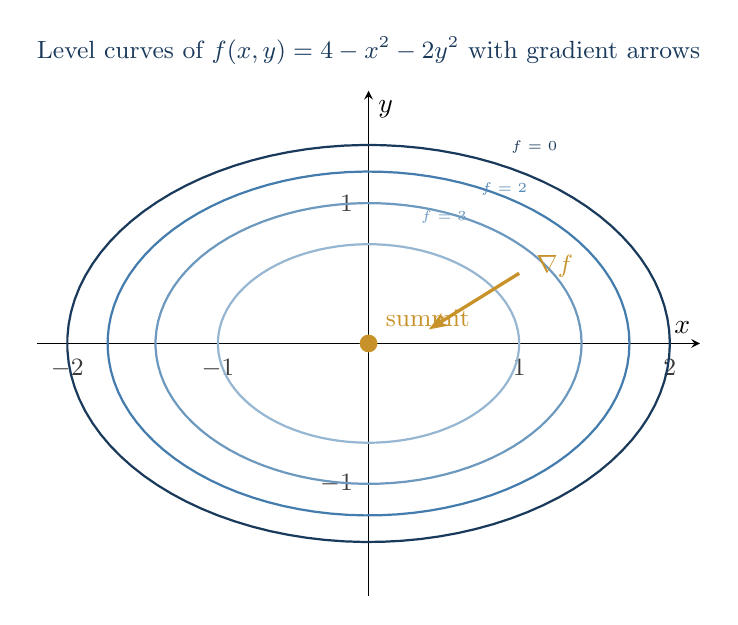
\begin{tikzpicture}
\begin{axis}[
  width=10cm, height=8cm,
  axis lines=center,
  xlabel={$x$}, ylabel={$y$},
  xmin=-2.2, xmax=2.2, ymin=-1.8, ymax=1.8,
  xtick={-2,-1,1,2}, ytick={-1,1},
  tick label style={font=\small, color=DarkGrey},
  title={\small\color{NavyBlue}Level curves of $f(x,y)=4-x^2-2y^2$ with gradient arrows},
  view={0}{90},
]
% Level curves (ellipses): f = 4 - x^2 - 2y^2 = c => x^2/a^2 + y^2/b^2 = 1
% c=3: x^2 + 2y^2 = 1 => x^2/1 + y^2/0.5 = 1
\addplot[MidBlue!50, thick, domain=0:360, samples=100] ({cos(x)}, {sin(x)/sqrt(2)});
% c=2: x^2 + 2y^2 = 2
\addplot[MidBlue!70, thick, domain=0:360, samples=100] ({sqrt(2)*cos(x)}, {sin(x)});
% c=1: x^2 + 2y^2 = 3
\addplot[MidBlue!90, thick, domain=0:360, samples=100] ({sqrt(3)*cos(x)}, {sqrt(3/2)*sin(x)});
% c=0: x^2 + 2y^2 = 4
\addplot[NavyBlue, thick, domain=0:360, samples=100] ({2*cos(x)}, {sqrt(2)*sin(x)});
% Gradient arrow at (1, 0.5): grad = (-2, -2) -> steepest descent = (2, 2)/norm
% Gradient points toward origin (inward on each ellipse)
\draw[-{Stealth[length=7pt]}, Gold, very thick] (axis cs:1, 0.5) -- (axis cs:0.4, 0.1);
\node[Gold, font=\small, right] at (axis cs:1.05, 0.55) {$\nabla f$};
% Level curve labels
\node[MidBlue!70, font=\tiny] at (axis cs:0.5, 0.9) {$f=3$};
\node[MidBlue!80, font=\tiny] at (axis cs:0.9, 1.1) {$f=2$};
\node[NavyBlue, font=\tiny] at (axis cs:1.1, 1.4) {$f=0$};
% Summit
\addplot[only marks, mark=*, mark size=3pt, Gold] coordinates {(0,0)};
\node[Gold, font=\small, above right] at (axis cs:0.05, 0.05) {summit};
\end{axis}
\end{tikzpicture}
\end{center}

\subsection{Step 3: The multivariable chain rule}

\begin{problem}
\label{prob:chain_multi}
If $z = f(x,y)$ and both $x$ and $y$ depend on a parameter $t$, then
\[
  \frac{dz}{dt} = \frac{\partial f}{\partial x}\frac{dx}{dt} + \frac{\partial f}{\partial y}\frac{dy}{dt} = \nabla f \cdot \frac{d\mathbf{r}}{dt}.
\]
\begin{enumerate}[label=(\alph*), topsep=2pt]
  \item Verify this formula for $z = x^2 + y^2$ with $x = \cos t$, $y = \sin t$ (motion around the unit circle). Compute $\frac{dz}{dt}$ directly and via the chain rule.
  \item A particle moves along a path $(x(t), y(t))$ on a temperature field $T(x,y)$. Express the rate of change of the particle's temperature $\frac{dT}{dt}$ in terms of the gradient and the velocity vector.
  \item For $z = f(x,y)$ with $x = g(s,t)$ and $y = h(s,t)$: write $\frac{\partial z}{\partial s}$ and $\frac{\partial z}{\partial t}$.
  \item \textbf{Implicit differentiation revisited.} If $F(x,y) = 0$ defines $y$ implicitly as a function of $x$, use the multivariable chain rule to derive $\frac{dy}{dx} = -\frac{\partial F/\partial x}{\partial F/\partial y}$. Compare with Module~2.
  \item Show that a function $f(x,y)$ is constant along a level curve $f = c$ if and only if the tangent to the curve is perpendicular to $\nabla f$. This proves geometrically that the gradient is always perpendicular to level curves.
\end{enumerate}
\end{problem}

\subsection{Step 4: Critical points in higher dimensions}

\begin{problem}
\label{prob:multi_optim}
A critical point of $f(x,y)$ occurs where $\nabla f = \mathbf{0}$, i.e.\ where both partial derivatives vanish.
\begin{enumerate}[label=(\alph*), topsep=2pt]
  \item Find all critical points of $f(x,y) = x^3 + y^3 - 3xy$.
  \item The nature of a critical point is determined by the \textbf{Hessian matrix} $H = \begin{pmatrix} f_{xx} & f_{xy} \\ f_{xy} & f_{yy} \end{pmatrix}$. At a critical point: if $\det H > 0$ and $f_{xx} > 0$, it's a local minimum; if $\det H > 0$ and $f_{xx} < 0$, a local maximum; if $\det H < 0$, a \textbf{saddle point}. Apply this to the critical points from (a).
  \item A saddle point is a point that is a local minimum in one direction but a local maximum in another. Sketch such a surface. Give a physical example of a saddle point in a potential energy landscape.
  \item \textbf{Lagrange multipliers.} To maximise $f(x,y)$ subject to $g(x,y) = 0$, the condition is $\nabla f = \lambda \nabla g$ for some scalar $\lambda$. Explain geometrically why this must hold at the maximum.
  \item Use Lagrange multipliers to find the maximum of $f(x,y) = xy$ subject to $x + y = 10$. Verify by substitution.
\end{enumerate}
\end{problem}

\begin{thought}
\textbf{Lagrange multipliers and constrained optimisation.}
The Lagrange multiplier condition $\nabla f = \lambda \nabla g$ says: at the constrained optimum, the gradient of the objective is parallel to the gradient of the constraint. Geometrically, the level curves of $f$ and the constraint curve $g = 0$ are tangent to each other. If they were crossing, you could move along $g = 0$ to increase $f$, so the point could not be optimal. This geometric argument is worth understanding deeply --- it underpins constrained optimisation in economics (utility maximisation subject to a budget), physics (energy minimisation subject to conservation laws), and machine learning (loss minimisation subject to model constraints).
\end{thought}

\subsection{Step 5: Multiple integrals}

\begin{problem}
\label{prob:double_int}
The \textbf{double integral} $\iint_R f(x,y)\,dA$ is the volume under $z = f(x,y)$ over the region $R$.
\begin{enumerate}[label=(\alph*), topsep=2pt]
  \item Interpret $\iint_R 1\,dA$. What does this measure?
  \item For $f(x,y) = x + y$ over the rectangle $R = [0,1]\times[0,2]$, compute the integral as an iterated integral: $\int_0^2\left(\int_0^1 (x+y)\,dx\right)dy$. Reverse the order: $\int_0^1\left(\int_0^2 (x+y)\,dy\right)dx$. Do you get the same answer?
  \item Compute $\iint_R (x^2 + y^2)\,dA$ where $R$ is the disc $x^2 + y^2 \leq 1$. Switch to polar coordinates $x = r\cos\theta$, $y = r\sin\theta$, $dA = r\,dr\,d\theta$.
  \item The average value of $f$ over $R$ is $\frac{\iint_R f\,dA}{\text{Area}(R)}$. Compute the average value of $x^2 + y^2$ over the unit disc.
  \item The double integral reduces to a product of single integrals when $f(x,y) = g(x)h(y)$ and $R$ is a rectangle: $\iint_R f\,dA = \left(\int g\,dx\right)\left(\int h\,dy\right)$. Prove this and use it to evaluate $\iint_{[0,1]^2} e^{x+y}\,dA$.
\end{enumerate}
\end{problem}

\begin{problem}
\label{prob:gradient_theorem}
The gradient, divergence, and curl are the building blocks of vector calculus.
\begin{enumerate}[label=(\alph*), topsep=2pt]
  \item For a vector field $\mathbf{F}(x,y,z) = (P, Q, R)$, the \textbf{divergence} is $\nabla \cdot \mathbf{F} = \frac{\partial P}{\partial x} + \frac{\partial Q}{\partial y} + \frac{\partial R}{\partial z}$. Compute $\nabla \cdot \mathbf{F}$ for $\mathbf{F} = (x^2, y^2, z^2)$. Interpret: what does positive divergence mean for a fluid flow?
  \item The \textbf{curl} is $\nabla \times \mathbf{F} = \left(\frac{\partial R}{\partial y} - \frac{\partial Q}{\partial z},\; \frac{\partial P}{\partial z} - \frac{\partial R}{\partial x},\; \frac{\partial Q}{\partial x} - \frac{\partial P}{\partial y}\right)$. Compute $\nabla\times\mathbf{F}$ for $\mathbf{F} = (-y, x, 0)$. Interpret.
  \item \textbf{Green's theorem} (2D): $\oint_C (P\,dx + Q\,dy) = \iint_R \left(\frac{\partial Q}{\partial x} - \frac{\partial P}{\partial y}\right)dA$. Use it to compute the area of a region $R$ using the line integral $\oint_C x\,dy$.
  \item \textbf{Gauss's theorem} (divergence theorem): $\iint_S \mathbf{F}\cdot d\mathbf{A} = \iiint_V (\nabla\cdot\mathbf{F})\,dV$. Interpret: the total flux out of a volume equals the integral of divergence inside it.
  \item All three theorems (Green, Stokes, Gauss) are special cases of one master theorem: $\int_{\partial\Omega} \omega = \int_\Omega d\omega$ (Stokes' theorem in differential forms). What does it say at the highest level of abstraction?
\end{enumerate}
\end{problem}

% ============================================================
\section{Part 3 \texorpdfstring{---}{--} Discovery}
% ============================================================

\begin{discoverybox}
\textbf{What have we built?}

\textbf{First.} The derivative in higher dimensions is the gradient $\nabla f$ --- a vector that points in the direction of steepest increase and is perpendicular to every level surface.

\textbf{Second.} The multivariable chain rule $\frac{dz}{dt} = \nabla f \cdot \frac{d\mathbf{r}}{dt}$ unifies all rate-of-change computations: the derivative of $f$ along a curve is the dot product of the gradient with the velocity.

\textbf{Third.} Optimisation extends naturally: critical points are where $\nabla f = 0$; the Hessian matrix classifies them; Lagrange multipliers handle constraints.

\textbf{Fourth.} The divergence theorem and Stokes' theorem are higher-dimensional analogues of the Fundamental Theorem of Calculus: they relate an integral over a region to an integral over its boundary. They are all special cases of one abstract theorem.

\medskip
\textbf{Looking back at Journey 2.} You have built the entire edifice of single and multivariable calculus from one question: what is the rate of change of a function at a point? The derivative answered it. The integral reversed it. Differential equations used it to describe the laws of nature. The gradient extended it to space.

\medskip
\textbf{The seed for Journey 3.} The gradient $\nabla f$ is a vector. The Hessian $H$ is a matrix. The divergence theorem involves volumes and surfaces. All of this requires \emph{linear algebra} --- the mathematics of vectors, matrices, and the transformations between them. Journey~3 will build that language from scratch, and return to everything in this module to understand it more deeply.
\end{discoverybox}

% ============================================================
\section{Part 4 \texorpdfstring{---}{--} Naming the Ideas}
% ============================================================

\begin{namebox}
\textbf{Partial derivatives and the gradient.}

For $f : \mathbb{R}^n \to \mathbb{R}$, the \textbf{partial derivative} $\frac{\partial f}{\partial x_i}$ is the derivative with respect to $x_i$ holding all other variables fixed.

The \textbf{gradient} is $\nabla f = \left(\frac{\partial f}{\partial x_1}, \ldots, \frac{\partial f}{\partial x_n}\right)$.

The \textbf{directional derivative} in direction $\hat{u}$ is $D_{\hat{u}} f = \nabla f \cdot \hat{u}$, maximised when $\hat{u} \parallel \nabla f$.

The gradient is perpendicular to every level surface $f = c$.
\end{namebox}

\begin{namebox}
\textbf{Critical points and the Hessian.}

A \textbf{critical point} satisfies $\nabla f = \mathbf{0}$. Classification via the Hessian matrix $H_{ij} = \frac{\partial^2 f}{\partial x_i \partial x_j}$:

At a critical point in $\mathbb{R}^2$: local min if $\det H > 0$ and $f_{xx} > 0$; local max if $\det H > 0$ and $f_{xx} < 0$; saddle if $\det H < 0$.

\textbf{Lagrange multipliers}: to optimise $f$ subject to $g = 0$, solve $\nabla f = \lambda \nabla g$ and $g = 0$.
\end{namebox}

\begin{namebox}
\textbf{The great theorems of vector calculus.}

\textbf{Green's theorem} (2D): $\oint_C P\,dx + Q\,dy = \iint_R \left(\frac{\partial Q}{\partial x} - \frac{\partial P}{\partial y}\right)dA$

\textbf{Stokes' theorem} (3D surface): $\oint_{\partial S} \mathbf{F}\cdot d\mathbf{r} = \iint_S (\nabla\times\mathbf{F})\cdot d\mathbf{A}$

\textbf{Gauss's theorem} (3D volume): $\iint_{\partial V} \mathbf{F}\cdot d\mathbf{A} = \iiint_V (\nabla\cdot\mathbf{F})\,dV$

All three are instances of $\int_{\partial\Omega} \omega = \int_{\Omega} d\omega$ (generalised Stokes' theorem in differential geometry).
\end{namebox}

% ============================================================
\section{Part 5 \texorpdfstring{---}{--} Deep Problems}
% ============================================================

\begin{deepproblem}[The total derivative as a linear map]
\begin{enumerate}[label=(\alph*)]
  \item The \emph{total derivative} of $f:\mathbb{R}^n\to\mathbb{R}$ at $\mathbf{x}_0$ is defined as the linear map $Df(\mathbf{x}_0):\mathbb{R}^n\to\mathbb{R}$ such that $f(\mathbf{x}_0 + \mathbf{h}) = f(\mathbf{x}_0) + Df(\mathbf{x}_0)\mathbf{h} + o(\|\mathbf{h}\|)$. Show that if $Df(\mathbf{x}_0)$ exists, it equals the row vector $(\nabla f)^T$.
  \item For $f:\mathbb{R}^n\to\mathbb{R}^m$, the total derivative $Df(\mathbf{x}_0)$ is an $m\times n$ matrix called the \textbf{Jacobian}. Compute the Jacobian of $f(x,y) = (x^2 + y, \sin(xy))$.
  \item The chain rule in this language is $D(f\circ g)(\mathbf{x}) = Df(g(\mathbf{x}))\cdot Dg(\mathbf{x})$ --- matrix multiplication. Show this reduces to the single-variable chain rule when $n = m = 1$.
  \item The \textbf{Inverse Function Theorem} in $\mathbb{R}^n$: if $Df(\mathbf{x}_0)$ is invertible, then $f$ is locally invertible near $\mathbf{x}_0$ and $(f^{-1})'(f(\mathbf{x}_0)) = [Df(\mathbf{x}_0)]^{-1}$. State what this means geometrically for a map $f:\mathbb{R}^2\to\mathbb{R}^2$.
\end{enumerate}
\end{deepproblem}

\begin{deepproblem}[Maxwell's equations]
Maxwell's four equations in vacuum describe all of electromagnetism:
\[
  \nabla\cdot\mathbf{E} = \frac{\rho}{\varepsilon_0}, \quad
  \nabla\cdot\mathbf{B} = 0, \quad
  \nabla\times\mathbf{E} = -\frac{\partial\mathbf{B}}{\partial t}, \quad
  \nabla\times\mathbf{B} = \mu_0\mathbf{J} + \mu_0\varepsilon_0\frac{\partial\mathbf{E}}{\partial t}.
\]
\begin{enumerate}[label=(\alph*)]
  \item Interpret each equation using the physical meanings of divergence and curl. What does $\nabla\cdot\mathbf{B}=0$ say about magnetic monopoles?
  \item In free space ($\rho = 0$, $\mathbf{J} = 0$), take the curl of the third equation and use the identity $\nabla\times(\nabla\times\mathbf{E}) = \nabla(\nabla\cdot\mathbf{E}) - \nabla^2\mathbf{E}$ to derive the wave equation $\nabla^2\mathbf{E} = \mu_0\varepsilon_0\frac{\partial^2\mathbf{E}}{\partial t^2}$.
  \item Identify the wave speed from the equation in (b). What is $1/\sqrt{\mu_0\varepsilon_0}$? What did Maxwell conclude in 1865?
  \item The wave equation has plane wave solutions $\mathbf{E} = \mathbf{E}_0 e^{i(\mathbf{k}\cdot\mathbf{r} - \omega t)}$. Substitute and find the dispersion relation between $\omega$ and $|\mathbf{k}|$.
  \item The mathematical structure of Maxwell's equations --- divergence and curl of vector fields, connected by the wave equation --- is a direct application of everything in this module. Write two sentences connecting the mathematics of multivariable calculus to the physics of light.
\end{enumerate}
\end{deepproblem}

\begin{deepproblem}[Differential forms and the generalised Stokes theorem]
A \textbf{differential 1-form} is an expression $\omega = P\,dx + Q\,dy$. Its \textbf{exterior derivative} is $d\omega = \left(\frac{\partial Q}{\partial x} - \frac{\partial P}{\partial y}\right)dx\wedge dy$.
\begin{enumerate}[label=(\alph*)]
  \item Show that Green's theorem reads $\int_{\partial R}\omega = \int_R d\omega$.
  \item A \textbf{closed form} satisfies $d\omega = 0$; an \textbf{exact form} satisfies $\omega = df$ for some function $f$. Show every exact form is closed. Is every closed form exact?
  \item Compute $d\omega$ for $\omega = \frac{-y\,dx + x\,dy}{x^2 + y^2}$ (defined for $(x,y)\neq(0,0)$). Show $d\omega = 0$. But show $\oint_C \omega = 2\pi \neq 0$ for any simple closed curve around the origin. What does this tell you about exactness?
  \item The failure of a closed form to be exact is measured by the \textbf{de Rham cohomology} of the space. The form in (c) shows $H^1(\mathbb{R}^2\setminus\{0\}) \neq 0$. What topological feature of $\mathbb{R}^2\setminus\{0\}$ does this reflect?
  \item \textit{(Preview of Journey 4 Module 2.)} The generalised Stokes theorem $\int_{\partial\Omega}\omega = \int_\Omega d\omega$ holds on any smooth manifold. Green's, Stokes', and Gauss's theorems are all special cases. What does this say about the relationship between the boundary of a space and the interior?
\end{enumerate}
\end{deepproblem}

% ============================================================
\section{Part 6 \texorpdfstring{---}{--} Reflection}
% ============================================================

\begin{reflectionbox}
\textbf{Final reflection for Journey 2.}

\begin{enumerate}
  \item \textbf{On the gradient.} In one variable, the derivative is a number. In $n$ variables, it becomes a vector. What is it in function space (infinitely many variables)? In the space of functions, the ``gradient'' of a functional (a function of functions) is called the \emph{functional derivative} --- and it governs the calculus of variations and quantum field theory. Write one sentence guessing what the gradient of a functional $F[f] = \int f(x)^2\,dx$ might mean.

  \item \textbf{On Maxwell's equations.} Maxwell derived the wave equation from his equations in 1865 and recognised the predicted speed as the speed of light, concluding that light is an electromagnetic wave. He had never set out to explain light --- he was doing mathematics. Write a paragraph: is this an example of mathematics predicting reality, or of mathematics being shaped by reality so that it was bound to predict it?

  \item \textbf{On boundary and interior.} The great theorems of vector calculus all say: an integral over the interior of a region equals an integral over its boundary. This is the Fundamental Theorem of Calculus in disguise. Write down the one-variable FTC and state what it says about boundary ($\{a, b\}$) and interior ($[a,b]$) in this language.

  \item \textbf{What Journey 2 built.} List five specific problems from real physics or engineering that Journey 2 has given you the tools to solve. Be specific: name the equation, the technique, and the application.
\end{enumerate}
\end{reflectionbox}

\medskip

\begin{namebox}
\textbf{What Journey 2 built.}

\medskip
\begin{center}
\renewcommand{\arraystretch}{1.5}
\begin{tabular}{l l l}
\toprule
\textbf{Module} & \textbf{Core discovery} & \textbf{What it enabled} \\
\midrule
1 & Derivative as limit & Instantaneous rate, tangent line \\
2 & Differentiation rules & Differentiating any combination efficiently \\
3 & Integral, FTC & Area, accumulated change, anti-differentiation \\
4 & MVT, optimisation & Shape of functions, maximum/minimum problems \\
5 & Differential equations & Physical laws as equations; ODE solution methods \\
6 & Gradient, vector calculus & Change in space; Maxwell, divergence theorem \\
\bottomrule
\end{tabular}
\end{center}

\medskip
Every result here feeds forward. The gradient is the foundation of Journey~3 (vectors and matrices). Differential equations and their solution spaces are the motivation for Journey~3's linear algebra. The wave equation connects to Journey~6's Fourier analysis. The generalised Stokes theorem connects to Journey~7's differential geometry.

You have not finished these ideas. You are midway through them.
\end{namebox}

\vspace{1.4cm}
\begin{center}
{\color{Gold}\rule{0.6\linewidth}{1.2pt}}\\[8pt]
{\large\bfseries\color{NavyBlue}End of Journey 2: Change}\\[6pt]
{\normalsize\color{DarkGrey}\itshape Six modules. Derivatives, integrals, ODEs, and the geometry of change in space.}\\[10pt]
{\color{Gold}\rule{0.6\linewidth}{1.2pt}}\\[10pt]
{\small\color{DarkGrey}Continue to: \textbf{Journey 3 --- Linear Structure}}\\[4pt]
{\small\color{DarkGrey}\itshape ``The purpose of computing is insight, not numbers.''\\
\upshape --- Richard Hamming}
\end{center}

\end{document}